\section[MODELO DE ARQUITETURA]{MODELO DE ARQUITETURA}

O modelo de arquitetura no seu nível mais elevado, pode ser visto como um modelo de três camadas, conforme a Figura \ref{camadas_arquitetura}.
\begin{figure}[ht]
	\centering
	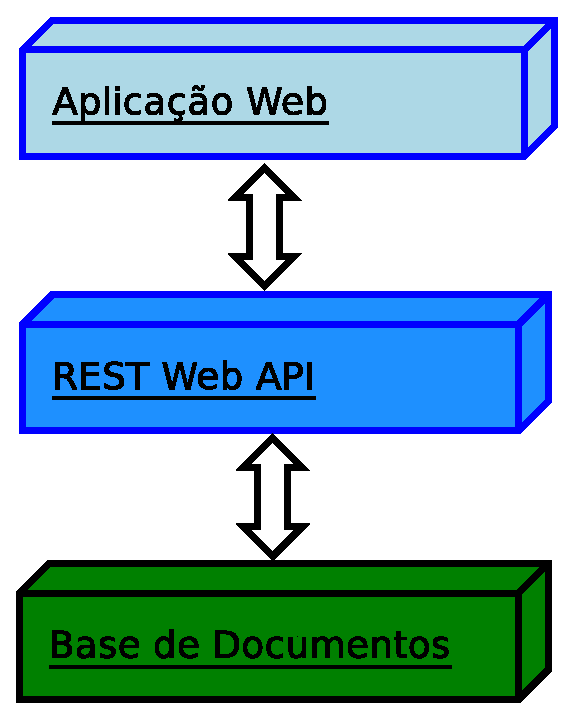
\includegraphics[width=7cm]{figuras/camadas.eps}
	\caption{Camadas arquiteturais}
	\label{camadas_arquitetura}
\end{figure}

A camada \emph{web} é responsável pela interação com o usuário. 
A camada \emph{Web API} é responsável pela lógica de negócio. 
A camada de base de documentos é responsável pela persistência dos dados da aplicação.


\subsection[CAMADA DE APLICAÇÃO WEB] {CAMADA DE APLICAÇÃO WEB}
Esta camada foi projetada para rodar em \emph{browsers} que suportam \emph{HTML} 5. 
Ela é desenvolvida usando-se \emph{Javascript}, \emph{CSS} e \emph{HTML}. 
Além disso, adotou-se o \emph{framework} de desenvolvimento \emph{web} \emph{AngularJS}. \textbf{ORGANIZAÇÃO DO CÓDIGO FONTE}

A criação de um ambiente de desenvolvimento \emph{web}, para um software de média para grande complexidade, não é uma tarefa trivial de ser resolvida.
É necessários criar padrões de organização de arquivos, configurar e instalar pacotes de software para desenvolvimento, testes, implantação, construção de builds, entre outros.
Para facilitar esta tarefa, optou-se em utilizar o projeto \emph{angular-seed}.
A ideia deste projeto é servir de esqueleto de projetos \emph{web} que utilizam o \emph{framework} \emph{AngularJS}.
Para usar este projeto basta cloná-lo diretamente do seu repositório \emph{git} no \emph{site} github.com, conforme o comando abaixo.
\lstset{language=bash}
\begin{lstlisting}[frame=single]
git clone https://github.com/angular/angular-seed.git
\end{lstlisting}

Antes de começar a usar o \emph{angular-seed} é necessário instalar o ambiente de execução \emph{Javascript Node.JS}. 
Este ambiente é utilizado para execução de testes e construção de \emph{builds}. Para uma introdução ao \emph{Node.JS} veja \cite{Syed2014}.


